\documentclass[T,J]{fose} % 「コンピュータソフトウェア」用のクラスファイルは compsoft です.
\taikai{2024} % 固定です.出版委員長が毎年変更してAuthor Kitを配布してください.

\usepackage [dvipdfmx] {graphicx}
\usepackage{xcolor} % 色を扱うためのパッケージ


% ユーザが定義したマクロなどはここに置く.ただし学会誌のスタイルの
% 再定義は原則として避けること.

\newcommand{\RQOne}{レビューコメントにおいて修正要求と修正確認は分類可能か}
\newcommand{\RQTwo}{レビューコメントにおいて修正完了の有無を分類することは可能か}
\newcommand{\RQThree}{PR単位と修正要求単位に基づく進捗状況評価結果は異なるか}

% 以下のマクロはサンプルファイル作成用のマクロです.不要であれば削除してください.
\newcommand{\todo}[1]{\colorbox{yellow}{{\bf TODO}:}{\color{red} {\textbf{[#1]}}}}
\newcommand{\change}[1]{\colorbox{green}{{\bf CHANGE}:}{\color{blue} {\textbf{[#1]}}}}
\newcommand{\new}[1]{\colorbox{cyan}{{\bf NEW}:}{\color{black} {\textbf{[#1]}}}}

% 利用しているパッケージのダウンロード.
\usepackage{amsmath}
\usepackage{fancyvrb}
\usepackage{url}
\usepackage{otf}

\begin{document}

% 論文のタイトル
\title{修正要求・確認コメントの自動抽出による \\ コードレビューの進捗状況追跡手法に向けて}
% 以下の \etitle(と\@etitle)はFOSE論文フォーマット独自のマクロです.
% FOSEに投稿した論文を発展させてコンピュータソフトウェアに投稿される場合はコメントアウトしてください.
% \setetitleは奇数ページのヘッダに表示する文字列(\etitle)を設定するためのマクロです.
% タイトルが2行に渡る場合は "\\" を 使用することで任意の位置で改行をすることができます.
\setetitle{Toward Tracking Code Review Progress by Extracting Modification Requests Comments and Confirmation Comments}
%\setetitle{Long Long Long Long Long Long \\ Long Long Long Long Long \\ Long Long Long Long Long Long Long Long Long Long Long Long Paper Title}

% タイトル,著者などが複数行にわたり,論文冒頭の著者名が日本語アブストと重複して描画された場合に以下のコメントアウトを外してください.
%\longtitle

% 著者
% 和文論文の場合,姓と名の間には半角スペースを入れ,
% 複数の著者の間は全角スペースで区切る
%
\author{川\UTF{FA11} 晴斗 伊原 彰紀 上中 瑞稀
%
% ここにタイトル英訳 (英文の場合は和訳) を書く.
% 英語タイトルは論文1ページ目左下,著者らの名前・所属一覧の一番上に表示される
%
% 上記\setetitle中で改行した場合は "\etitle" を削除し,改行(\\)を入れていないタイトルを記載してください.
% \ejtitleは1ページ目左下に挿入されるタイトルとして使用されます.
% また,"\etitle"はFOSE論文フォーマット独自のマクロです.
\ejtitle{\etitle}
%
% ここに著者英文表記 および
% 所属 (和文および英文) を書く.
% 複数著者の所属はまとめてよい
% 複数著者の所属は以下のようにまとめてよい.
\shozoku{Haruto Kawasaki, Akinori Ihara}{和歌山大学}
{Wakayama University}
}
%
% 和文アブストラクト
% In English paper, content of Jabstract will be ignored. 
\Jabstract{%
コードレビュー対象のソースコードが改善を要する場合,検証者は実装者に修正を要求する.ソフトウェア開発においてプロジェクト管理者は,コードレビューの進捗を確認しながら次のリリースに導入可能なソースコードを決定する.しかし大規模なプロジェクトでは,膨大なコードレビューの個々の進捗を確認することは容易ではない.本研究では,レビューコメントから修正要求コメント,および修正要求が解決されたことを示す修正確認コメントをそれぞれ自動抽出し,コードレビューの進捗状況を追跡する手法を提案する.%本手法の方が従来の進捗状況評価指標として用いられているレビューコメント票より進捗の変動を細かく表すことを確認した.\change{研究の結果}
%リポジトリへの導入には改善を要するソースコードは,検証者が実証者に修正を要求する.ソフトウェア開発プロジェクトでは,コードレビューの進捗状況を個別に確認しながら,次のリリースに導入するプロダクトを決定する.しかし,日々膨大なソースコードのコードレビューが依頼されると,個別の状況を確認することは容易でない.本研究では,レビューコメントから修正要求と,実装者による修正が問題ない修正確認を抽出し,それぞれを対応したコメント同士で紐づけることによりソースコードレビューの進捗状況を追跡する手法を提案する.
}

\maketitle \thispagestyle {empty}

%%%%%%%%%%%%%%%%%%%%%%%%%%%%%%%%%%%%%
\section{はじめに}
%%%%%%%%%%%%%%%%%%%%%%%%%%%%%%%%%%%%%

コードレビューは,機能追加や不具合修正のために開発者(実装者)が変更したソースコードを,別の開発者(検証者)が欠陥の有無やコードの可読性を確認する重要な工程である\cite{quality1}\cite{quality2}.特に不特定多数の実装者が参加するオープンソースソフトウェア (OSS) 開発には,多様なコーディングスタイルで実装されたソースコードが提出されるため,複数の検証者によってコードレビューが実施される~\cite{review_process}.コードレビューによってソースコードの改善を要する箇所が発見されれば,検証者は実装者に改善を要求する.

%オープンソースソフトウェア (OSS) 開発では日々ソースコードの変更提案を開発者(実装者)から受けている.今日ではソフトウェアの品質維持のために欠陥の有無やコードの可読性などを確認するコードレビューが重要であるということが示されている~\cite{Quality1}\cite{Quality2}ことからOSS開発でもコードレビューが行われることは多い.コードレビューは提出された変更提案に対して複数の開発者(検証者)によって行われ,プロジェクトに導入もしくは却下される他,ソースコードの修正を実装者へ求められることがある.

リリースまでのマイルストーンを計画するために,ソフトウェア開発プロジェクトはコードレビューを含めたタスクの進捗を計画し,進捗状況を追跡する~\cite{review_time}.GitHubが提供する機能であるMilestoneは,特定の期限までに完了する必要がある不具合 (Issue) 票やコードレビュー (Pull Request) 票の件数を把握することができ,多くの組織がスケジュールを検討するために使用している.各コードレビュー票の中には,ソースコードの改善要求が含まれ,改善要求を明確に提示できる作業タスクであれば,緻密なマイルストーンを計画することが可能である.しかし,コードレビューでは実装者や他の検証者とタスクとすべきか判断するために議論を要することも少なくなく,その結果,コードレビューの時間が長期化している~\cite{review_time1}~\cite{review_time2}.

本研究では,コードレビューにおける進捗状況の把握に向けた第一歩として,検証者がコードレビュー票に残したコメントの中から修正要求コメント,および確認コメントの自動抽出する手法を開発し,本手法を検証する.また,GitHubのMilestoneのようにコードレビューチケット数に基づく進捗管理と,本研究で開発する修正要求数に基づく進捗管理の違いを示す.

% 本研究では3つのResearch Questionに回答する.


% プロジェクトに集まる大量のを処理し、優先順位をつけることに問題があると報告している。
% Work Practices and Challenges in Pull-Based Development: The Contributor’s Perspective@ICSE2016
% https://dl.acm.org/doi/10.1145/2884781.2884826


% また,プロジェクト管理者は変更提案毎にレビューコメントを確認し,検証者から依頼されている修正要求とその修正要求の完了度合いを管理している.変更提案の進捗を管理することでプロジェクト管理者はリリース日から逆算して,必要な実装者や検証者にプロジェクトの参加を推薦している.

% しかし,大規模なプロジェクトではプロジェクト管理者がレビューコメントを読むことの可能な量よりも実装者によって提出された変更提案数に対するレビューコメントの量が上回ることもあり,それぞれの変更提案における進捗を管理することは難しい.そのため,変更提案毎の進捗をレビューコメントから自動抽出することはプロジェクト管理者にとって有意義ではあるが,修正要求の基準や修正要求に対して既に修正が完了しているか否かを判別する手法が存在しないため,進捗の自動抽出は可能ではない.

% そのため,修正要求の完了状況を自動で確認する手法が存在しないことから,プロジェクト管理者は進捗状況の追跡手法の代替手段として,提出されている変更提案の数を確認している.変更提案の総数を確認することで変更提案毎にかけられるコストを目算することが可能であるため,おおよその進捗状況を追跡することは可能である.しかし,修正要求の完了度合いを確認しているわけではないため,提出されている変更提案を確認するだけでは細かな進捗の変動を追跡することは難しい.

% そこで本研究では進捗の追跡に向けて,レビューコメントから修正要求を抽出し,抽出した修正要求に対して修正完了の可否を分類することが可能であるかを検証する.
% また,本論文では3つの調査質問について検証を行う.

\noindent\textbf{RQ1: \RQOne(\ref{sec:RQ1}章)}\\
RQ1では,検証者が記録するコードレビュー票に残したコメントを修正要求と修正要求が解決されたことを示す修正確認を分類できるか否かを目視調査する.具体的には,OSS開発で公開されているコードレビュー票を無作為抽出し,各コードレビュー票に記録されたレビューコメントを目視調査する.

\noindent\textbf{RQ2: \RQTwo(\ref{sec:RQ2}章)}\\
RQ2では,レビューコメントに対して修正要求や修正確認であるか否かを目視によって分類したデータセットを教師データとし,学習済みモデルBERTをファインチューニングすることで,修正要求や修正確認を分類するモデルを構築する.さらに,修正要求文とその要求が解決されたことを確認する修正確認文の紐づけを試みる.
%を使用して元にそれぞれを抽出する手法の提案と検証を行う.また,修正要求の完了度合いを算出するために,修正要求とその修正要求に対する修正確認を紐づける手法を提案し,紐づいた割合について確認する.

\noindent\textbf{RQ3: \RQThree(\ref{sec:RQ3}章)}\\
RQ3では,本研究で開発した修正要求コメント,および修正確認コメントの抽出によってコードレビューの進捗状況を追跡結果の違いを示す.
% 手法を用いることで従来のコードレビュー票での進捗状況評価指標では確認できなかった微量を把握できるか検証する.\change{RQ3説明文追加}

% RQ3では,本研究で作成した修正要求単位の進捗状況評価指標は従来の変更提案単位での進捗状況評価指標では確認できなかった微量の進捗を把握できるか検証する.

以降,本論文では,\ref{sec:progress}章でOSS開発における進捗確認方法と従来研究について述べる.その後,\ref{sec:RQ1}章でRQ1,\ref{sec:RQ2}章でRQ2,\ref{sec:RQ3}章でRQ3のそれぞれの手法と結果について述べる.そして\ref{sec:discussion}章で結果の考察及び妥当性について述べ,\ref{sec:conclusion}章でまとめる.



%%%%%%%%%%%%%%%%%%%%%%%%%%%%%%%%%%%%%
\section{関連研究}\label{sec:progress}
%%%%%%%%%%%%%%%%%%%%%%%%%%%%%%%%%%%%%

大規模OSSの開発では,実装者がコードレビュー依頼をGerritやReview Boardをはじめとしたコードレビュー管理システムの票に記録することで,実装者と検証者が円滑なコミュニケーションを行う~\cite{code_review}.これらのシステムに蓄積されたデータを用いて,コードレビューの作業内容や工数を見積もる研究が行われている.
% Peter C. Rigby and Christian Bird. 2013. Convergent contemporary software peer review practices. In Proceedings of the 2013 9th Joint Meeting on Foundations of Software Engineering (ESEC/FSE 2013). Association for Computing Machinery, New York, NY, USA, 202–212. https://doi.org/10.1145/2491411.2491444

% コードレビューはプロジェクトの品質を担保するために重要なプロセスである~\cite{Quality1}\cite{Quality2}.検証者は実装者によって提出された変更提案に対してレビューを行い,プロジェクトに導入や却下,または変更提案に対して実装者へ修正を求める.修正が求められた変更提案は実装者によって修正が行われ,再度検証を依頼することができる.この作業を繰り返し,全ての修正に対して対処が完了したことを確認した場合には検証者によってプロジェクトに導入される.

% プロジェクト管理者は変更提案に対するレビューを確認することで検証者によって依頼されている修正要求の量を把握している.修正要求の量を把握することでプロジェクトのリリースに合わせた実装者や検証者の推薦を行っている.


% \subsection{コードレビュー票の優先順位に関する研究}

大規模OSSの開発では,日々膨大なコードレビュー票がプロジェクトに提出されるため,開発者はコードレビューを実施するソースコードに優先順位をつけざるを得ない.従来研究では,優先的にコードレビューするソースコードの優先順位を決定するための研究が多数取り組まれている.具体的には,ソフトウェア利用者に悪影響を与えるセキュリティ関連のソースコード変更のコードレビューは優先順位が高く設定される~\cite{integrator}\cite{review_prioritize_pineapple}.しかし,その他の急を要さない不具合修正やリファクタリングのために変更されるソースコードのコードレビューは優先順位が日々変動する.Kononenkoらは,開発者へのインタビューにおいて,直近のリリースに導入する変更提案の優先順位はリリースまでの期間によって異なることを明らかにしている\cite{release_merge}.

コードレビューの進捗を計画,追跡することは,リリースまでの緻密なマイルストーンを計画するために重要であり,各コードレビューに要する時間を見積もる研究が行われている~\cite{estimate_time1}\cite{estimate_time2}\cite{estimate_time3}\cite{estimate_time4}\cite{estimate_time5}.
Maddilaらは,コードレビュー対象のソースコード行数,変更内容の種類,コードレビューチケット作成日,ソースコード作成者の特徴など28の特徴量に基づきコードレビュー時間を見積もる手法を提案している\cite{estimate_time2}.

コードレビューの優先順位,およびコードレビューにかかる工数の見積もりに関する従来研究では,コードレビューチケットを提出時に計測できる特徴量に基づいていることが多い.検証者による修正要求に基づき優先順位やコードレビューに要する時間を見積もることで,さらに正確なマイルストーンを計画することができると考える.そこで,本研究では修正要求コメント文を自動抽出する手法を開発し,コードレビューの進捗状況の追跡を試みる.


% \subsection{動機}
% 大規模なプロジェクトでは実装者から提出される変更提案数は膨大であるため,プロジェクト管理者がレビューコメントを確認することで変更提案毎の修正要求の進捗を把握することは現実的ではない.

% そこで本研究では変更提案における進捗を自動抽出するために,レビューコメントから修正要求と修正確認を抽出し,修正要求と修正確認を対応したコメント同士で紐づけることで,修正要求の抽出と修正要求の修正完了の可否を分類可能にすることを目指す.そのため,まずRQ1では,レビューコメントに対して目視調査を行い,修正要求と修正確認を分類可能かを確認する.次にRQ2では,レビューコメントから修正要求と修正確認の分類とそれぞれの紐付けを行うことで修正完了の有無を分類可能かを検証する.最後にRQ3では,本研究で作成した修正要求の進捗状況追跡手法は適切か,変更提案の進捗状況追跡手法との違いについて検証を行う.


%%%%%%%%%%%%%%%%%%%%%%%%%%%%%%%%%%%%%
\section{RQ1:\RQOne}\label{sec:RQ1}
%%%%%%%%%%%%%%%%%%%%%%%%%%%%%%%%%%%%%

\subsection{概要}
コードレビュー票には多数のコメントが記録されている.実装者が投稿するコメントでは,作成したソースコードの補足,検証者からの質問に対する回答などがある.検証者が投稿するコメントでは,実装者への修正要求,提出されたパッチへの問い,修正要求が解決完了の確認などがある.RQ1では,コードレビュー票に記録されたコメントの中から,修正要求と修正要求が解決されたことを示す修正確認を分類できるか否かを目視調査する.

% 変更提案における進捗を自動抽出するために,レビューコメントから修正要求の完了状況を抽出する必要がある.そこでRQ1では,レビューコメントを目視で調査し,修正要求や修正完了の分類が可能であるかの目処を立てる.具体的には,データセットのうち一部のレビューコメントに対して修正要求や修正確認であるか否かを著者二人で議論を行い,分類を行う.得られたデータセットを元に修正要求や修正確認に特徴はあるのか考察する.

\subsection{データセット}
RQ1では,OpenStackのコアコンポーネントであるNova,Neutron,Cinder,Keystone,Swift,Glanceの6つのプロジェクト,およびOpenStackにおける大規模プロジェクトであるHorizonの合計7つのプロジェクトを分析対象とし,各プロジェクトにおいて立ち上げ時から2022年9月までにリポジトリに導入されたコードレビュー票に記録されるコメントを収集する.表
\ref{table:NumberOfProjects}は,各プロジェクトのコードレビュー票数,コメント数を示す.プロジェクト毎のコードレビュー票の平均コメント数は22件から87件である.

%-----------------------
\begin{table}[t]
\centering
  \caption{各プロジェクトにおいて導入されたコードレビュー票数とコメント数}
  \label{table:NumberOfProjects}
  \scalebox{0.95}{   
  \begin{tabular}{l|r|r}  \hline \hline
    \multicolumn{1}{c|}{プロジェクト} & \multicolumn{1}{c|}{コードレビュー票数} & \multicolumn{1}{c}{コメント数}\\ \hline
    Nova & 29,338 & 1,571,114\\ \hline
    Neutron & 18,665 & 1,106,829\\ \hline
    Cinder & 12,917 & 1,127,176\\ \hline
    Horizon & 9,645 & 209,681\\ \hline
    Keystone & 8,270 & 190,464\\ \hline
    Swift & 6,172 & 112,709\\ \hline
    Glance & 4,545 & 102,360\\ \hline
  \end{tabular}
  }
\end{table}
%-----------------------

\subsection{手法}
分析対象とする7プロジェクトを区別せずに89,552件のコードレビュー票から信頼区間95\%,許容誤差5\%となる383件を無作為に選択し,コードレビュー票に投稿されたコメント12,086件を目視調査する.具体的には,修正要求のコメント,および修正確認のコメントを抽出する.ただし,ボットによるテスト実行結果は修正要求,修正確認と判定しない.

%のコードレビュー票に含まれる12,086件のレビューコメントを無作為に抽出した.抽出したレビューコメントに対して著者二人が議論を行い,変更提案のレビューコメント毎に「修正要求か否か」と「修正確認か否か」という二つの観点において分類した.また,分類の際に修正要求や修正確認に特徴があるのか調査する.

\subsection{結果}
12,086件のレビューコメントのうち,874件が修正要求であり,1,874件が修正確認であることを確認した.

%-----------------------
\begin{table*}[t]
\centering
  \caption{修正要求に含まれていた内容}
  \label{table:request_sum}
  \scalebox{0.85}{   
  \begin{tabular}{l|l|r}  \hline \hline
    \multicolumn{1}{c|}{修正要求内容} & \multicolumn{1}{c|}{コメント例} & \multicolumn{1}{c}{件数(重複可)}\\ \hline
    機能改善 & better to use mock instead of stub & 297\\ \hline
    リファクタリング/コード整形 & could remove these variables if un-used & 278\\ \hline
    コード外の修正(コミットメッセージ等) & commit message line should have less than 72 characters & 233\\ \hline
    バグ & need to address failures in unit tests & 92\\ \hline
    機能追加 & conf.register\_group(wsgi\_group)' should be added & 69\\ \hline
    typo & fileds -\textgreater fields & 47\\ \hline
  \end{tabular}
  }

\vspace{2mm}

\centering
  \caption{修正確認に含まれていた内容}
  \label{table:achieve_sum}
  \scalebox{0.9}{   
  \begin{tabular}{l|l|l}  \hline \hline
    \multicolumn{1}{c|}{修正確認内容} & \multicolumn{1}{|c}{コメント} & \multicolumn{1}{|c}{件数(重複無)} \\ \hline
    強い承認 & Looks good to me, approved または Code-Review+2 & 666 \\ \hline
    弱い承認 & Looks good to me, but someone else must approve または Code-Review+1 & 893 \\ \hline
    その他 & Good Change や Thank you や Nice など & 315 \\
    % & I would prefer this is not submitted as is または \\ Code-Review-1 & 弱い非承認 \\ \hline
    % This shall not be submitted または \\ Code-Review-2& 強い非承認 \\ 
    \hline
  \end{tabular}
  }
\end{table*}
%-----------------------

表~\ref{table:request_sum}は,修正要求を内容に基づき分類した結果を示す.本分析では,6つの修正要求に分類することができ,機能改善,リファクタリング,コード外の修正の順で修正要求されていることがわかった.\todo{できれば複数事例書いて,コメントには類似しているものがあることを書きたい}

% 修正要求の内容の種類は多岐にわたることはなく,6つの種類で分類することができた.また,分類された件数が多い修正要求内容の上位3つは下位3つと比べて件数が十分に多いことがわかる.このことから,修正要求の内容の種類の分布は小さいことがわかる.また,修正要求は例に示しているように内容を直接的に伝えるような記述のされ方が多く,皮肉や質問を交えた修正要求が提案されることは少ないことを確認した.\change{表2の内容を記述}

著者が修正確認として判断したコメントのうち,83.2\%はOpenStackで提供されている変更提案に対する承認を表す検証評価ラベルがレビューコメントに付与されていることを確認した.検証評価ラベルはGerritで提供される機能の一つで,コードレビュー結果をスコアで評価を提示することができる.表\ref{table:achieve_sum}に示す強い承認または,弱い承認を表すコメントは検証評価ラベルである.また,Gerritの機能ではなく,検証者がコメントとして``Good Change''や``Thank you''などを投稿していることも確認した.

また,修正要求が修正確認と紐づいているかの実情を確認した結果,修正要求を提出した検証者が後に修正確認をしていないこともあり,修正要求と修正確認が一対一対応していないことも存在していた.

%である.OpenStackではこれのラベルを付けることで変更提案に対して承認/非承認を行うことが可能であることから,高い割合でラベルが付いていたということが考えられる.

これらの結果からレビューコメントにおける修正要求または,修正確認には特徴があることを確認したため,修正要求や修正確認は機械的な手法でレビューコメントから抽出できることが示唆される.

%%%%%%%%%%%%%%%%%%%%%%%%%%%%%%%%%%%%%
\section{RQ2:\RQTwo}\label{sec:RQ2}
%%%%%%%%%%%%%%%%%%%%%%%%%%%%%%%%%%%%%

\subsection{概要}
RQ2では,学習済みモデルBERTをファインチューニングすることで,レビューコメントに修正要求,および修正確認を含むか否かを機械的に特定する手法を提案し,評価する.

%レビューコメント,を抽出することが可能であるかを検証し,修正確認と修正要求を対応したコメント同士で紐づけることで修正要求の修正が完了しているか否かを分類することが可能であるかを検証する.

\subsection{手法}
% 本節では,レビューコメントから修正要求を抽出する手法と修正確認を抽出する手法を示す.


\subsubsection{修正要求の抽出}
\ref{sec:RQ1}章で目視調査したデータセットを教師データとして用い,自然言語モデルBERT\footnote{BERT: \url{https://huggingface.co/docs/transformers/ja/model_doc/bert}}をファインチューニングしたモデルでレビューコメントに修正要求を含むか否か判定する.目視調査した12,086件を5分割し,一つをテスト用のデータに用いて,残りの4つ分のデータを訓練,検証に7:3の割合で分割する5分割交差検証を行う.モデル作成時のパラメータは学習時のパッチサイズが8,評価時のパッチサイズが16,エポック数が3,ウォームアップステップ数が500,重み減衰が0.01とした.また,評価指標には5回の駆動の中央値の適合率,再現率,F1値を用いる.

% \ref{sec:RQ1}章で目視調査したデータセットを教師データとして用い,自然言語モデルBERT\footnote{BERT: \url{https://huggingface.co/docs/transformers/ja/model_doc/bert}}をファインチューニングしたモデルでレビューコメントに修正要求を含むか否か判定する.目視調査した12,086件のレビューコメントを訓練\todo{追加学習?}用,検証用に7:3の割合で分割する.設定したパラメータは,学習時のパッチサイズが8,評価時のパッチサイズが16,エポック数が3,ウォームアップステップ数が500,ウェイトディケイが0.01とする.\todo{これらの設定は何に従う?}
% %次に分割したデータセットを元に自然言語処理モデルのBERTにファインチューニングを行う.設定したパラメータは,学習時のパッチが8,評価時のパッチサイズが16,エポック数が3,ウォームアップステップ数が500,ウェイトディ系が0.01である.この修正要求を抽出する用のモデルを用いて元のデータセットから修正要求を抽出する.
% また,構築したモデルの評価を行うために別途\ref{sec:RQ1}章で分類したデータセットを5分割し,一つをテスト用のデータに用いて,残りのデータを訓練,検証に7:3の割合で分割する5分割交差検証を行なった.\todo{先ほどの訓練と検証とは違う?7:3で5分割交差検証したら2回評価するコメントがでてきてしまう.8:2の間違い?}モデル作成時のパラメータは先ほど説明したパラメータと同一である.また,評価指標には5回の駆動の平均の適合率,再現率,F1値を用いる.

\subsection{修正要求と修正確認の紐付け}
RQ1において,目視によって修正要求と修正確認を紐づけ可能な事例も存在したが,紐付けが容易でない事例も存在していた.そこで本研究では進捗状況評価を行うための第一歩として,修正要求コメントの投稿後に提出された修正確認コメント(``LGTM'',``Looks good'',``Looks ok'')に全て紐づける.

% 修正要求と修正確認を紐づけるために目視調査を行い,修正要求の内容と修正確認の内容が紐づく条件を確認した.その結果,修正要求と,修正要求が提出されたパッチより後に存在する修正確認は紐づくことを確認できた.

% 3.4章の結果から修正確認と分類されたレビューコメントのうち83.2\%は承認を表すラベルがコメントに含まれていることを確認した.また,修正確認と分類したコメントのうち,修正確認として用いられているフレーズを抽出した.次に,それらのフレーズにおいて著者によって修正確認として判別された回数を出現回数で除算する式\ref{eq:confidence}を用いてフレーズの修正確認としての信頼度を算出する.

% \begin{equation}\label{eq:confidence}
% \text{信頼度} = \frac{\text{フレーズが修正確認として判別された回数}}{\text{フレーズの総出現回数}}
% \end{equation}

% 信頼度が90\%を超えたコメントは``LGTM'',``Looks good'',``Looks ok''であったことから,本研究では承認を表すラベルの他にも,これらの3つのフレーズが含まれているレビューコメントを修正確認として扱い,修正確認として判別されたレビューコメントの網羅率を検証する.

% % RQ1おいて,個々の修正要求が,個別に修正確認と紐づく事例以外にも,個別に確認されない事例も少なからず存在していることを確認した.このケースに対応するため,本研究では要求後にいずれかの検証者による確認が取れれば,それまでの要求は全て確認されたものとみなす.

% 確認される場合は,3.4章の結果から修正確認と分類されたレビューコメントのうち83.2\%は承認を表すラベルが合わせて付けられていることを確認した.また,修正確認と分類したコメントのうち,修正確認として用いられているフレーズに対するコメントの信頼度を調査したところ,``LGTM'',``Looks good'',``Looks ok''が90\%を超えていたことから,本研究では承認を表すラベルか信頼度が90\%を超える3つのいずれかがついているレビューコメントを修正確認として扱い,修正確認として分類されているコメントの網羅率を検証する.

% また,RQ1において個別に修正要求が確認されない場合も多いため,本研究では,そのようなケースは要求後にいずれかの検証者による確認がとれれば,それまでの要求はすべて確認されたものとみなす.確認は要求を出した人が確認するという方法もあるがノイズが入るため,今後の課題とする.

% この修正要求と修正確認を紐づけるための条件を用いて修正要求と修正確認を紐付け,各プロジェクトにおいて修正要求の紐づいた割合を算出する.

\subsection{結果}
検証用に作成したモデルを用いた修正要求の5分割交差検証の結果は中央値の適合率が0.84,再現率0.85,F1値0.86となった.この結果から修正要求は高い割合で予測可能であることが示唆される.

次に,承認を表すラベルか信頼度が90\%を超えコメントのいずれかが含まれているコメントを修正確認として扱ったところ,レビューコメントのうち修正確認として分類されたコメントの97.3\%を修正確認として分類可能なことを確認した.

最後に,修正要求の抽出用に作成したモデルを用いた.目視調査した12,086件のレビューコメントを訓練用,検証用に7:3の割合で分割してモデルを構築し,89,552件の変更提案から239,286件の修正要求を抽出した.また,定義した修正要求が提出されたパッチより後に存在する修正確認と紐付けを行ったところ207,111件が紐づくことを確認した.

%%%%%%%%%%%%%%%%%%%%%%%%%%%%%%%%%%%%%
\section{RQ3:\RQThree}\label{sec:RQ3}
%%%%%%%%%%%%%%%%%%%%%%%%%%%%%%%%%%%%%

\subsection{概要}
RQ2ではデータセットに対して修正要求と修正確認を抽出し,それぞれを対応したコメント同士で紐付けを行なった.RQ3では従来の進捗状況評価指標で用いられるコードレビュー票の件数と修正要求の件数での進捗状況評価では特徴が異なるかを検証する.

\subsection{分析手法}
3.3章のデータセットを用いて,1日毎に存在したコードレビュー票の件数と修正要求の件数の分布に有意差が存在するかを検証する.

%変更提案単位と修正要求単位での進捗状況評価の違いを確認するため,開放されている変更提案と未完了の修正要求の数の推移を確認する.まず,変更提案単位では変更提案が開放されると加算し,プロジェクトに導入されると減算を行い,その時点に開放されている変更提案の推移を示す.次に,修正要求単位では修正要求が提出されると加算し,修正確認と紐づく場合に減算を行う.また,変更提案がプロジェクトに導入された場合には全ての修正要求が満たされたと仮定して変更提案に含まれる紐づいていない修正要求の数だけ減算する.


%\subsection{データセット}

%3.3章のデータセットを用い,PR単位の推移を測る際には,変更提案毎の開放時間を用いる.また,修正要求や紐付け手法に関しては4章で解説したものを用いる.

\subsection{結果}
1日毎に存在したコードレビュー票の件数と修正要求の件数の分布を図\ref{fig:task_dist}に示す.全てのプロジェクトで有意差があり,コードレビュー票の件数と修正要求の件数の分布が異なることを確認した.

また,全てのプロジェクトで効果量を測定したところ,Keystoneが0.47という最も高い値を算出したため,Keystoneのコードレビュー票の開放数の推移と修正要求の開放数の推移を図~\ref{fig:task_trans}に示す.修正要求はコードレビュー票と比べて開放数の変動が大きく,コードレビュー票を確認するだけでは追跡できなかった進捗状況を追跡可能であることが示唆される.

%-------------------
\begin{figure}[t]
\centerline{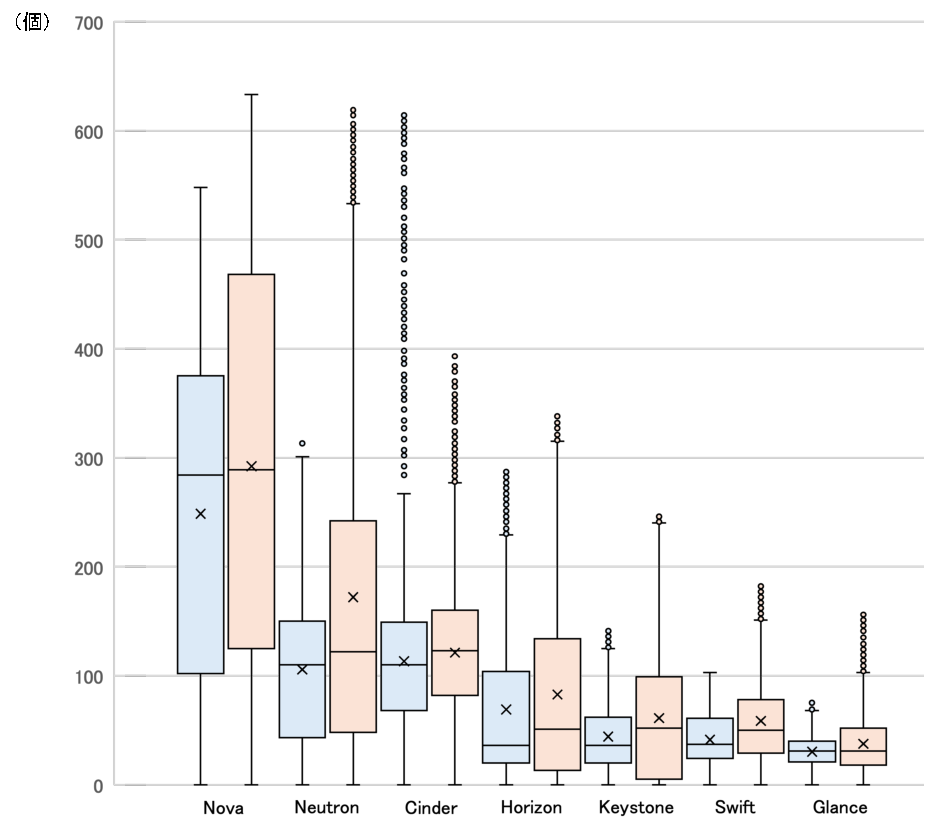
\includegraphics[width=1.0\linewidth]{Kawasaki_fig/task_dist.pdf}}
\caption{1日毎の存在するコードレビュー票の件数と修正要求の件数の分布(左:コードレビュー票, 右:修正要求)}
\label{fig:task_dist}

\vspace{2mm}

\centerline{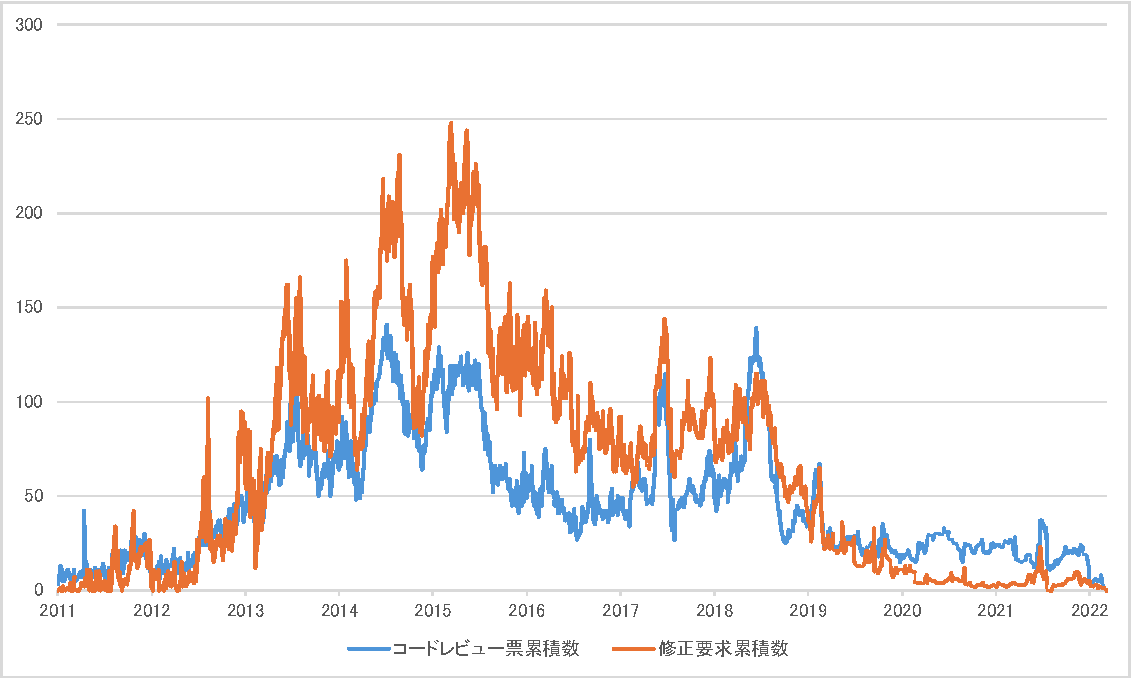
\includegraphics[width=1.0\linewidth]{Kawasaki_fig/task_trans.pdf}}
\caption{Keystoneのコードレビュー票と修正要求の開放数の推移}
\label{fig:task_trans}
\end{figure}
%-------------------

%%%%%%%%%%%%%%%%%%%%%%%%%%%%%%%%%%%%%
\section{考察}\label{sec:discussion}
%%%%%%%%%%%%%%%%%%%%%%%%%%%%%%%%%%%%%

\subsection{RQ3の考察を行う予定}


%\subsection{妥当性の脅威}
%\subsubsection{内的要因}
%本研究では,修正要求や修正確認の基準を作成するために,データセットの一部に対して目視で修正要求か否かと修正確認か否かを分類した.

%\subsubsection{外的要因}
%本研究では,7つのOSSプロジェクトを対象に分析を行った.対象となるプロジェクトを変更することで,本研究での結果と異なる可能性がある.そのため,本研究では,多くの変更提案が提出されているプロジェクトを選択することで,脅威を削減する.

%%%%%%%%%%%%%%%%%%%%%%%%%%%%%%%%%%%%%
\section{おわりに}\label{sec:conclusion}
%%%%%%%%%%%%%%%%%%%%%%%%%%%%%%%%%%%%%


%================
%\section*{参考文献}
%================
\bibliographystyle{junsrt}
\bibliography{KawasakiFOSE}

\end{document}